\documentclass{standalone}
\usepackage{tikz}
\usetikzlibrary{intersections,calc,fadings,decorations.pathreplacing,shapes.geometric}
\usepackage{verbatim}
\usepackage{xparse}
\usepackage{wasysym}

\begin{document}

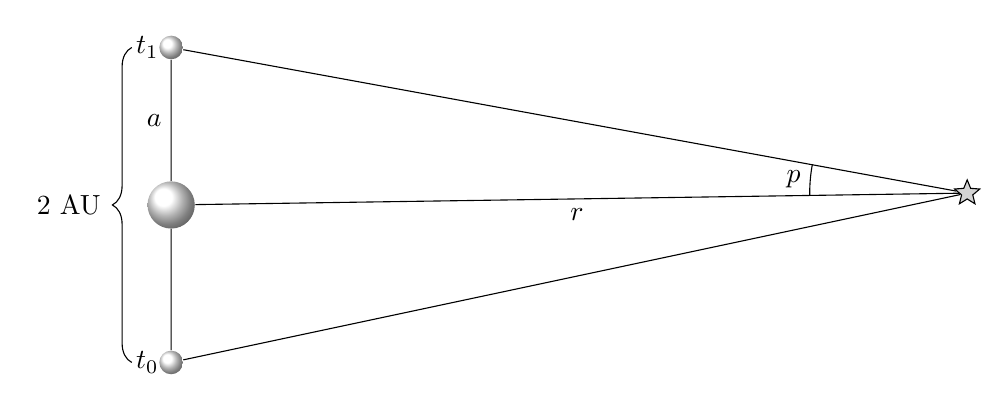
\begin{tikzpicture}
	[bigdot/.style={circle,ball color=white,fill opacity=1,inner sep=0pt,minimum size=0.6cm},
		smalldot/.style={circle,ball color=white,fill opacity=1,inner sep=0pt,minimum
		size=0.3cm}]
%	star/.style={star,star points=5,star point ratio=2.25,color=gray,draw,inner
%	sep=1.3pt,anchor=outer point 3}]
		\tikzstyle{stars}=[star,star points=5,star point ratio=2.25,fill=gray,fill
			opacity=0.35,
			draw,inner sep=1.5pt,anchor=outer point 3]

	\node (sun) at (0,0)  [bigdot] {};
	\node (t1) at (0,-2) [smalldot] {};
	\node[left=1pt] at (0,-2) {$t_0$};
	\node (t2) at (0,2) [smalldot] {};
	\node[left=1pt] at (0,2) {$t_1$};
	\node (star) at (10,0) [stars] {};
%	\node (5,0) (star) {};
	\draw (t1) -- (sun) to node[left] {$a$} (t2) -- (star) -- (t1);
	\draw (sun) to node[below] (sun-to-star) {$r$} (star);

	\draw[decorate,decoration={brace,amplitude=7pt},xshift=-0.5cm,yshift=0cm]
	(0,-2) -- (0,2) node [midway,xshift=-0.8cm] {2 AU};

	\begin{scope}[shift={(star)}]
		\draw (181:2) arc (181:169.5:2);
%		\draw (180:2) arc (180:170:2);
		\node[left] (parallax) at (175:2) {$p$};

%		\draw (181+11:3) arc (181+11:169.5:3);
	\end{scope}
%	\draw (5,0) (180:1) arc (180:170:1);
%	\node at (0,0) [circle] 

%	\filldraw[ball color=yellow, fill opacity=1] (0,0) circle [radius=0.5cm] node(sun)
%	{};
%	\filldraw[ball color=blue, fill opacity=0.5] (0,3) circle [radius=0.1cm] node(t2)
%	{};
%	\filldraw[ball color=blue, fill opacity=0.5] (0,-3) circle	[radius=0.1cm]
%	node(t1) {};

%	\node[draw, circle, ball color=white, fill opacity=1] (sun) at (0,0) [radius=0.5cm] {};

%	\draw (t1) -- (sun) -- (t2);
%	\draw (t1.north) -- (sun.south);
%	\draw (sun.north) -- (t2.south);
	
	





\end{tikzpicture}

\end{document}
